\section{Experiment}
\label{sec:experiment}


To verify the effectiveness of the Matching The Statements model, we conduct extensive experiments on the ArgKP-2021 \citep{bar-haim-etal-2020-arguments} dataset and compare the performance of MTS against baselines. 

\subsection{ArgKP-2021 Dataset}

ArgKP-2021 \citep{bar-haim-etal-2020-arguments}, the data set used in the Quantitative Summarization – Key Point Analysis Shared Task, is split into training and development sets with the ratio of $24:4$. The training set is composed of 5583 arguments and 207 key points while those figures in the development set are 932 and 36. Each argument could be matched to one or more key points, yet the latter ones account for a small proportion of the data, as stated in section \ref{sec:prepare}. The texts presented in ArgKP-2021 are relatively short, with approximately $18.22 \pm 7.76$ by words or $108.20 \pm 43.51$ by characters.

\subsection{Evaluation protocol}

For evaluation, only the most likely key point is chosen for each argument based on the predicted scores. These pairs are then sorted by their matching scores in descending order, and only the first half of them are included in the assessment. According to \citet{kpa-2021-overview}, there are two metrics used in Track 1, namely relaxed and strict mean Average Precision (mAP):
\begin{align*}
\mathbf{Precision} = \frac{\mathrm{True\:Positive}}
{\mathrm{True\:Positive} + \mathrm{False\:Positive}}
\end{align*}

Since there are some argument-key point pairs in the ArgKP-2021 dataset that have indecisive annotations (i.e. their label is neither matched nor non-matched): in the relaxed mAP evaluation, these pairs are considered as matched whereas strict mAP treats them as non-matched pairs.

\begin{figure}[ht]
\centering
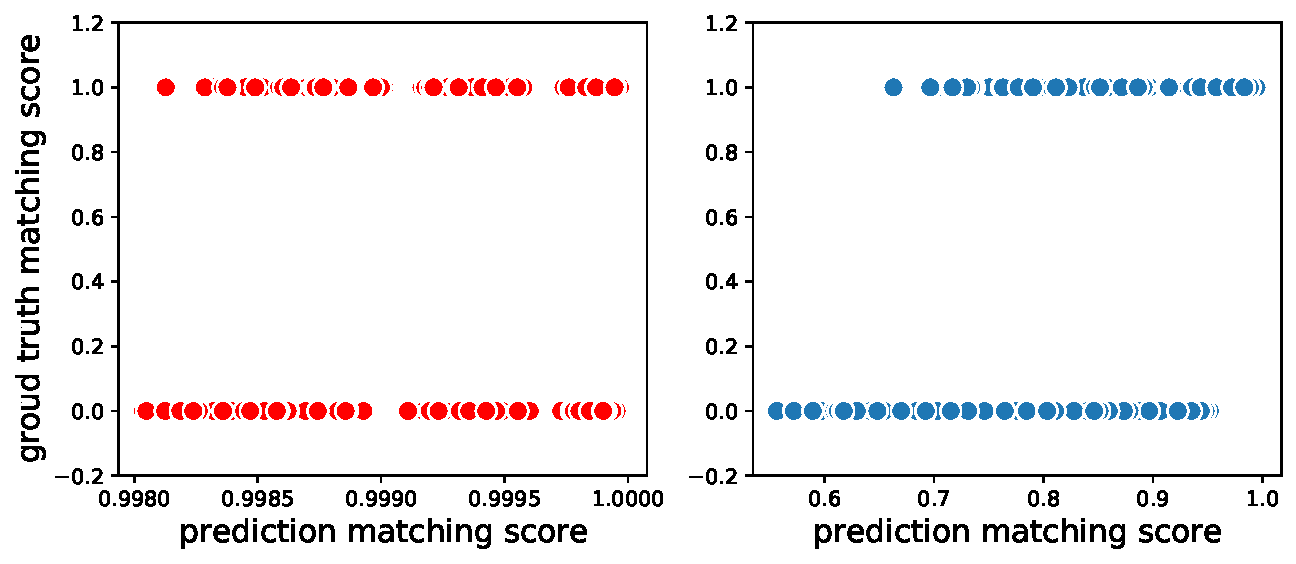
\includegraphics[scale=0.35]{figures/before-after.pdf}
\caption{Statement representation before (left) and after (right) training.}
\label{fig:before-after}
\end{figure}

\subsection{Embeddings quality}

Figure \ref{fig:before-after} depicts the qualitative representation learning result of MTS before and after training. In the beginning, the similarity scores between matched/non-match key point-argument pairs are extremely high ($\approx0.999$). That means, almost all the statements are projected into a small region of the embedding space, and it is difficult to derive a cut-off threshold to get rid of the non-matching pairs.

Therefore, the mean Average Precision scores when we directly use the untrained model with RoBERTa backbone are relatively low. Though, our training procedure improves the model's distinguishability and reduces the collapsed representation phenomenon. Indeed, the similarity scores at this point are stretched out and the mAP scores significantly increase ($\text{strict\:mAP}\;0.45\to0.84;\\ \text{relaxed\:mAP}\:0.62\to0.94$).

\begin{figure}[t]
\centering
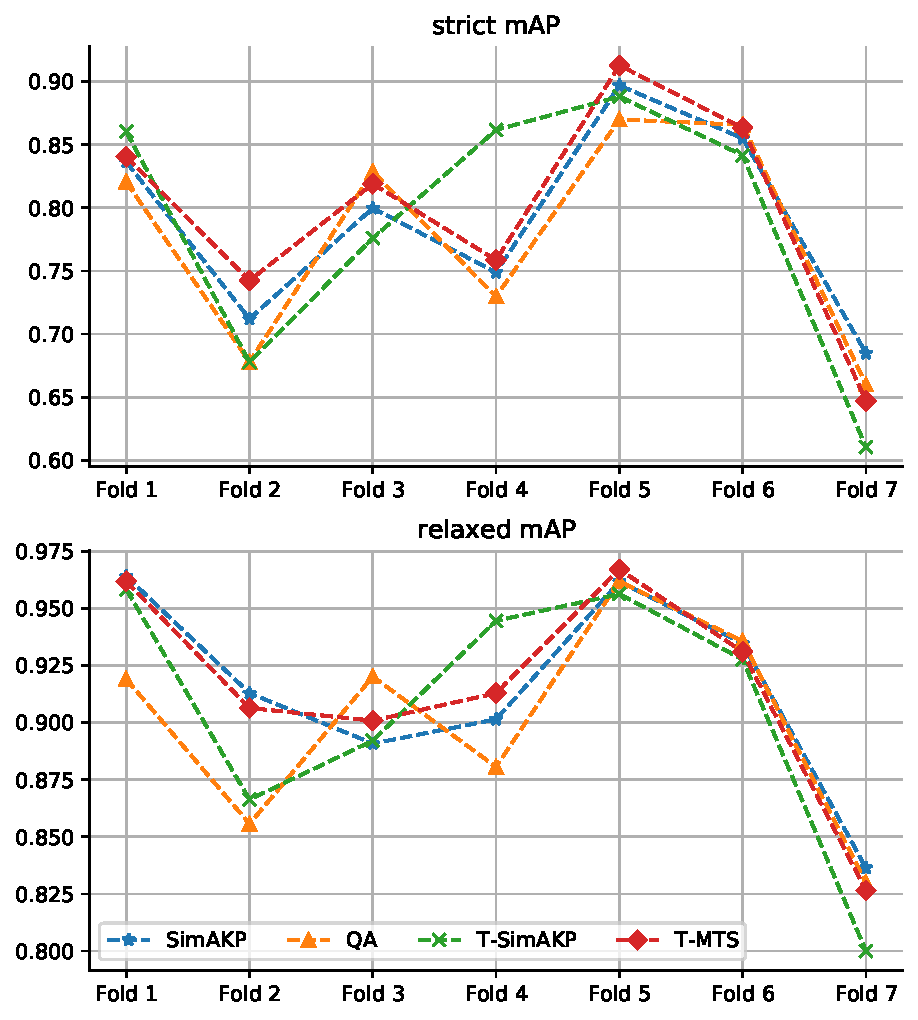
\includegraphics[scale=0.49]{figures/7-folds.pdf}
\caption{Mean Average Precision scores over 7 folds. The "T-" prefix denotes the models that use triplet loss \citep{dong2018triplet} while the rest are trained with the contrastive loss \citep{chopra2005learning}.}
\label{fig:7-folds}
\end{figure}

\subsection{Baselines}

For performance benchmarking, we implement two different baselines and their variations, namely Simple Argument-Key point matching (SimAKP) and Question Answering-liked Argument-Key point matching (QA) models. We construct a sampling strategy in an online manner: in each mini-batch, we select the hardest positive/negative pairs according to the method discussed in Section \ref{sec:training} to compute the loss.

\textbf{Simple Argument-Key point matching:} The architecture of SimAKP is the same as MTS with the main difference in the data preparation. Instead of clustering similar statements, SimAKP simply performs pair-wise classification on the ArgKP-2021 dataset. Equivalently, each input to the SimAKP model consists of an argument-key point pair. This approach will not make use of the analogous nature of these claims that matched with the same key point.

\textbf{Question Answering-liked Argument-Key point matching:} Inspired by the Question Answering, we format the arguments and key points fed to the RoBERTa model in order to incorporate the context into statements as below:

\hspace*{3mm}[CLS] Topic [SEP] [SEP] Statement [SEP]

\hspace*{3mm}[CLS] Topic  [SEP] [SEP] Key point [SEP]

where [CLS] and [SEP] are two special tokens.

In particular, obtained outputs of RoBERTa model with the above inputs are then concatenated with the stance representations to produce a tensor with shape $(\mathrm{batch\:size}, N+3072)$, which is fed to a fully connected layer to embed the semantic meaning of each individual statement.
\subsection{Results}

To facilitate evaluation, we set up a 7-fold cross-validation, each contains 24 topics for training and 4 topics for development. The train-dev split in Track 1 of Quantitative Summarization – Key Point Analysis Shared Task is replicated in fold 1.

As can be seen in Figure \ref{fig:7-folds}, we observe that our proposed MTS (we use triplet loss for a fair comparison) consistently outperforms other baselines in both mAP scores (higher is better). It achieved competitive scores on all splits, except fold 7. The reason is that the number of labeled argument-key point pairs of the development set in this part is the smallest among 7 folds, and there are substantial drops in terms of performance for all baselines.
\begin{table}[ht]
\centering
\begin{tabular}{|c|c|c|}
\hline
\textbf{Model} & \textbf{strict mAP} & \textbf{relaxed mAP}\\
\hline\hline
    SimAKP 
    & $0.790 \pm 0.072$ & $0.914 \pm 0.041$   \\
    \begin{tabular}{@{}c@{}}SimAKP \\\noindent w.o mining\end{tabular} 
    & $0.783 \pm 0.074$ & $0.917 \pm 0.037$   \\
    T-SimAKP 
    & $0.788 \pm 0.098$ & $0.906 \pm 0.054$   \\
    \begin{tabular}{@{}c@{}}T-SimAKP \\\noindent w.o mining\end{tabular} 
    & $0.782 \pm 0.101$ & $0.901 \pm 0.076$   \\
\hline
\end{tabular}
\caption{\label{tab:hard-mining}
The effect of hard sample mining in baselines.
}
\end{table}

We also examine the impact of hard negative mining in Table \ref{tab:hard-mining}, the baselines are compared against themselves when using the hard mining strategy (i.e. avoid learning the embeddings of trivial samples). With the employment of hard mining, there is an improvement in performance for most baselines. Except for a small decrease in terms of relaxed mAP in SimAKP, both contrastive and triplet loss Simple Argument-Key point matching models have an average increase of 0.005\% in mAP scores.

\subsection{Differential Analysis}
To provide insight analysis in the setting of Matching The Statements, we therefore create four different setups: original MTS, MTS with batch normalization \citep{ioffe2015batch} immediately after context integration layer, MTS without mining strategy, and triplet-loss MTS. Although tuplet margin loss has an up/down weighting hard/easy samples mechanism, we find that MTS with multi-similarity mining \citep{wang2019multi} performed best during the exploratory phase. 

\begin{figure}[h]
\centering
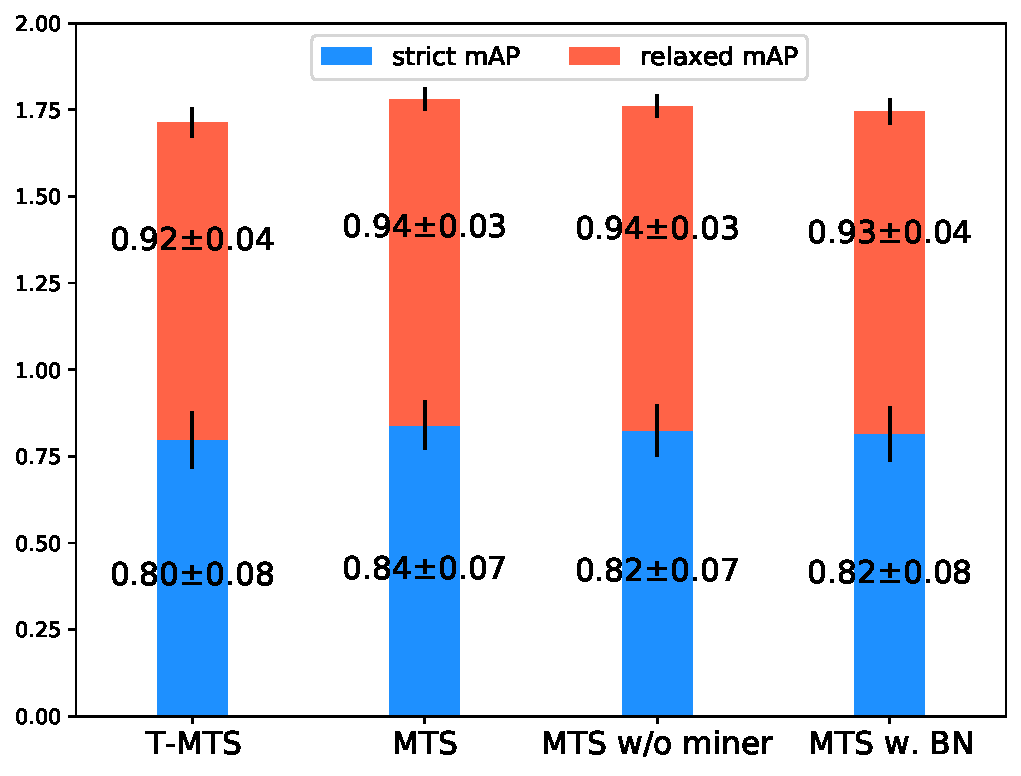
\includegraphics[scale=0.44]{figures/modification.pdf}
\caption{Switching off different setups shows that each component of the original MTS's setting contributes to its performance.}
\label{fig:modification}
\end{figure}

Figure \ref{fig:modification} summarizes the average score for all setups. Overall, MTS performs similarly or better than its variants (without multi-similarity mining or adding a batch normalization layer). Replacing triplet loss with tuplet margin loss helps to boost both strict mAP and relaxed mAP by 0.2. Eventually, in an attempt to produce a consistent and accurate prediction on the test dataset, an ensemble of 4/7 best models from splits was used for final submission. As shown in Table \ref{tab:leaderboard}, among the performances of the top-10 team, our proposed model achieved the third position in terms of strict mAP, $7^{th}$ position in relaxed mAP and $4^{th}$ overall.
\begin{table}[ht]
\centering
\begin{tabular}{|P{3mm}|P{22mm}|P{17mm}|P{17mm}|}
\hline
\textbf{\#} & \textbf{Team} & \textbf{strict mAP} & \textbf{relaxed mAP}\\
\hline\hline
    $1$ & mspl & $0.908\:(2)$ & $0.972\:(3)$   \\
    $2$ & heinrichreimer & $0.912\:(1)$ & $0.967\:(5)$   \\
    $3$ & vund & $0.878\:(4)$ & $0.968\:(4)$   \\
    $\mathbf{4}$ & \textbf{HKL\:(ours)} & $\mathbf{0.896\:(3)}$ & $\mathbf{0.963\:(7)}$   \\
    $5$ & sohanpatnaik & $0.872\:(5)$ & $0.966\:(6)$   \\
    $6$ & fengdoudou & $0.853\:(10)$ & $0.98\:(2)$   \\
    $7$ & mozhiwen & $0.833\:(12)$ & $0.985\:(1)$   \\
    $8$ & Fibelkorn & $0.869\:(6$ & $0.952\:(10)$   \\
    $8$ & emanuele.c & $0.868\:(7)$ & $0.956\:(9)$   \\
    $10$ & niksss & $0.858\:(8)$ & $0.95\:(11)$   \\
\hline
\end{tabular}
\caption{\label{tab:leaderboard}
Leaderboard of the Track 1 Quantitative Summarization – Key Point Analysis.
}
\end{table}
\subsubsection{BERT embeddings}
\label{sec:bert_emb}

\begin{table*}[t]
\centering
\begin{tabular}{|c|c|c|c|}
\hline
\textbf{Embedding} & \textbf{strict mAP} & \textbf{relaxed mAP} & \textbf{\#Param}\\
\hline\hline
    {Sum all tokens}
    & $0.834 \pm 0.065$ & $0.938 \pm0.037$  & \multirow{3}*{$125$M}\\
    {Mean all tokens}
    & $0.796 \pm 0.068$ & $0.916 \pm0.034$  & \\
    {[CLS] last hidden layer}
    & $0.823 \pm 0.072$ & $0.937 \pm0.038$  & \\ 
    \textbf{[CLS] 4 hidden layers}
    & $\mathbf{0.840 \pm 0.071}$ & $\mathbf{0.941 \pm0.034}$  & {$126$M} \\
\hline
    LUKE
    & $0.808 \pm 0.096$ & $0.926 \pm0.056$  & $276$M \\
    ALBERT
    & $0.748 \pm 0.071$ & $0.879 \pm0.044$  & $13$M \\
    MPNet
    & $0.839 \pm 0.059$ & $0.940 \pm0.029$  & $111$M \\
    DistilBERT 
    & $0.724 \pm 0.065$ & $0.864 \pm0.058$  & $68$M \\
    BERT (uncased)
    & $0.746 \pm 0.062$ & $0.888 \pm0.035$  & \multirow{2}*{$110$M} \\
    BERT (cased)
    & $0.752 \pm 0.073$ & $0.883 \pm0.057$  &  \\
\hline
\end{tabular}
\caption{\label{tab:bert-embedd}
Comparison between different embedding strategies and pre-trained language models. In this experiment, we report the result of the base version.
}
\end{table*}
Here, we showcase the benefit of taking the concatenation of the last four hidden state layers of the [CLS] token as the aggregate representation for the whole document. The first part of Table \ref{tab:bert-embedd} is a clear proof for this advantage, using only the last hidden layer of [CLS] can hurt the overall performance. Likewise, the mean-pooling or summing up the token embeddings has worse results, compared to our method. 

To show the generality and applicability of our proposed model, we retain the MTS configuration when experimenting with other transformers-based backbones, such as: BERT \citep{devlin2018bert}, ALBERT \citep{lan2019albert}, DistilBERT \citep{sanh2019distilbert}, LUKE \citep{yamada2020luke} or MPNet \citep{song2020mpnet}. According to the second part of Table \ref{tab:bert-embedd}, among six pre-trained language models, MPNet yields a comparable result with RoBERTa ($\approx0.84\:\&\:0.94$) while requiring $10\%$ less number of parameters. We also note that, the increase in model size of Language Understanding with Knowledge-based Embeddings (LUKE) compared with RoBERTa results in unexpected performance reduction.
\subsubsection{Stance effect}
\label{sec:stance}
Up till now, we have almost finished the needed experiments to examine the effectiveness of our methodology. In this subsection, we further investigate the importance of the stance factor in building the MTS model by posing a question: \textit{"How good is MTS when it has to predict the implicit relation between claims and topic"}. Since the topic information is incorporated in encoding the statements, so perhaps it is sufficient to learn meaningful representations, without explicitly providing the stance information.

By discarding the stance-involved components in MTS \ref{fig:model}, the averaged result in 7 folds conceivably degrades to $0.741\pm0.094$ in strict mAP but rises up to $0.952\pm0.019$ in relaxed mAP. This is because each argument now can be matched with key points that have different stances. According to this exploration, an open challenge for future research is finding a better way to comprehend statements within a topic (i.e. let the model infer the stance itself). For instance, one could consider employing the attention mechanism between a topic and its arguments and key points to characterize the relationship between them.

\section{Conclusion}
\label{sec:conclusion}

In this paper, we present an efficient key point matching method based on supervised contrastive learning. We suppose that clustering the statements will be beneficial for the model training, and empirically verify this conclusion in the experiments. In addition, we found a simple and effective technique to encode these statements, and thus yields superior performance. In terms of model architecture, the components are carefully designed to ensure productivity. Results on Track 1 of Quantitative Summarization – Key Point Analysis show our method is a conceptually simple approach yet achieves promising performance.